We used a questionnaire to understand the current experiences of interaction between
SCs and their ESPs. We restricted the analysis to sites in the United States
because the results of the survey and practices of DR are are highly
correlated and driven by energy policies in the country. 
\cite{torriti_demand_2010}.

Nineteen Top100 List sized sites in the United States were targeted for the
questionnaire. Eleven sites responded---Oak Ridge National Laboratory (ORNL), 
Lawrence Livermore National Laboratory, 
Argonne National Laboratory (ANL), 
Los Alamos National Laboratory (LANL), 
Lawrence Berkeley National Laboratory (LBNL), 
Wright Patterson Air Force Base,
National Oceanic Atmospheric Administration (NOAA), 
National Center for Supercomputing Applications (NSCA), 
San Diego Supercomputing Center (SDSC), 
Purdue University and Intel Corporation. The questionnaire was
sent to a sample that was not randomly selected. It was sent to those sites
where it was relatively easy to identify an individual based on membership
within the EE HPC WG. The sample is more representative of Top50 sized sites
(One Top50 sized site was not in the sample and 60{\%} (9/15) of the sample
responded). Only 4 additional sites were sampled from the Top51-Top100 List
and, of those, 2 responded (Intel and NOAA).
%Patki: New Graph instead of Table 1
\begin{figure}[htbp]
\begin{center}
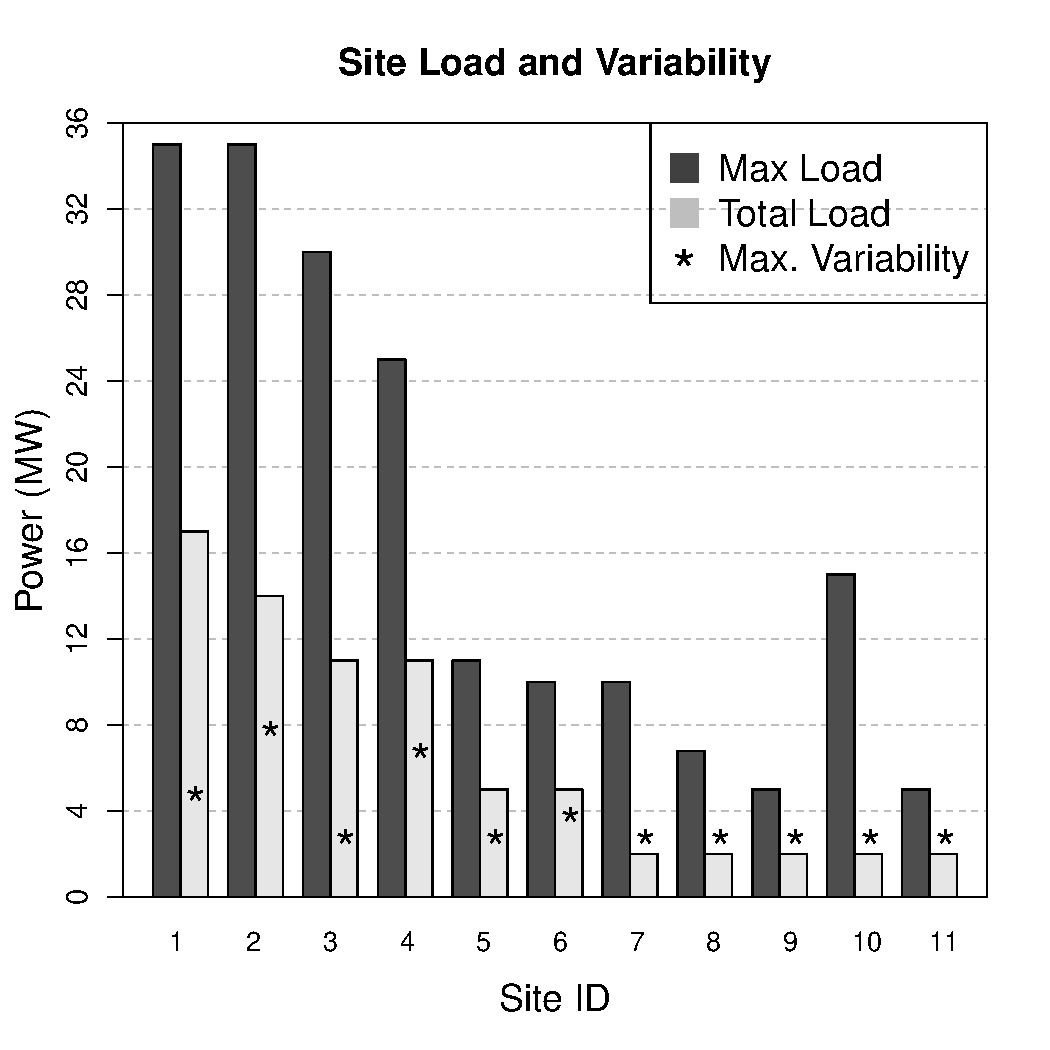
\includegraphics[scale=0.45]{NewGraphs/Table1-graph.pdf}
\caption{Site Load and Variability}
\label{figGraph1}
\end{center}
\end{figure}

The total power load as well as the intra-hour fluctuation of these sites
varied significantly (Figure \ref{figGraph1}). Total power load includes all computing systems plus ancillary systems such as power delivery and cooling components.
There were four sites with total power load greater
than 10 MW, two sites with \textasciitilde5 MW total power load and five
sites with less than 2 MW  of total power load. For those with total power load greater than 10 MW, the
intra-hour fluctuation (maximum variability) varied from less than 3 MW to 8 MW. One of
\textasciitilde 5 MW sites said that they experienced 4 MW variability. We chose less than 3 MW intra-hour variability as the bottom of the scale because we assumed that the
ESPs would not be affected by 3 MW (or less) 
fluctuations. The rest of the sites all reported less than 3 MW intra-hour fluctuation. Most of the intra-hour variability was due to preventative maintenance. 
%TP: THis is repeated. (again, the power variation includes both computing and ancillary systems).

For every respondent, the theoretical peak energy or maximum load is approximately twice the total energy, which is indicative of expected future growth in power and energy requirements for SCs. Some of the design parameters that may affect theoretical peak limits are the customer switchgear, transformer 
and chiller water capacities. In some cases, there are also limits based on regional ESP capacity constraints.

We asked if the SCs had talked to their ESPs about programs and methods used to balance the grid supply and demand of electricity (see Table 1). About half of them have had some discussion, but it
has mostly been limited to programs (e.g., peak shed, dynamic pricing) 
and not methods (e.g., regulation, frequency response, congestion).

\begin{table}[htbp]
\caption{Discussions with ESPs}
\begin{tabular}{|p{190pt}|l|}
\hline
\textbf{Discussions with ESPs}&
{\%} Yes \\
\hline
\textbf{Demand-side programs}&
~ \\
\hline
Shedding load during peak demand&
54 \\
\hline
Responding to pricing incentive programs&
45 \\
\hline
Shifting load during peak demand&
36 \\
\hline
\textbf{Supply-side programs}&
~ \\
\hline
Enabling use of renewables&
36 \\
\hline
Congestion, Regulation, Frequency Response&
18 \\
\hline
Contributing to electrical grid storage&
10 \\
\hline
\end{tabular}
\label{tab2}
\end{table}

Approximately half of the respondents are not currently interested in shedding
load during peak demand. LANL reports that the ``technical feasibility" and ``business case has yet to be developed."
There is slightly more interest in shifting than shedding load. SDSC reports that
 ``Automatic load shedding is being explored/deployed today'' for the entire campus, not just the SC.

\begin{table*}[htbp]
\centering
\caption{HPC Strategies Responding to Electricity Provider Requests}
\begin{tabular}{|p{2.5in}|p{0.75in}|p{0.75in}|p{0.75in}|} \hline

\textbf{HPC strategies for responding to} &
\textbf{\%} &
\textbf{\%} &
\textbf{\%} \\

\textbf{Electricity Provider requests} &
\textbf{Interested} &
\textbf{High} &
\textbf{Medium} \\

\textbf{(listed from highest to lowest interest + impact)} &
 &
\textbf{Impact} & 
\textbf{Impact} \\
\hline

Coarse grained power management &
64 &
46 &
27 \\
\hline

Facility shutdown&
36 &
64 &
10 \\
\hline

Job scheduling&
36 &
27 &
18 \\
\hline

Load migration &
10 &
36 &
18 \\
\hline

Re-scheduling back-ups &
45 &
0 &
10 \\
\hline

Fine-grained power management &
27 &
0 &
36 \\
\hline

Temperature control beyond ASHRAE limits &
27 &
0 &
18 \\
\hline

Turn off lighting &
18 &
0 &
0 \\
\hline

Use back-up resources (e.g., generators) &
0 &
10 &
27 \\
\hline

\end{tabular}
\label{tab3}
\end{table*}
Responding to pricing incentive programs is also not considered currently interesting by approximately half of the respondents, although the reasons for this low interest may be organizational. Several
open-ended comments revealed that pricing is fixed and/or done by another
organization at the site level and outside of their immediate control.

Only twenty percent of the respondents have had discussions with their
ESPs about congestion, regulation and frequency
response. LANL is one of the two who have had discussions and who commented that
they are ``learning about the process'' and that it is ``outside of [their] visibility or control''.

There were many more respondents who have had discussions with their
ESPs about enabling the use of renewables; 36{\%}
have already had discussions and more than half are interested in further
and/or future discussions. SDSC already has a site-wide program; ``the
campus has a large fuel cell (2.5$+$ MW) and works with the utility with
renewables.'' Other responses suggest that the interest is at the site level
and not unique to the SC.

%Patki: Fig 2
\begin{figure}
\begin{center}
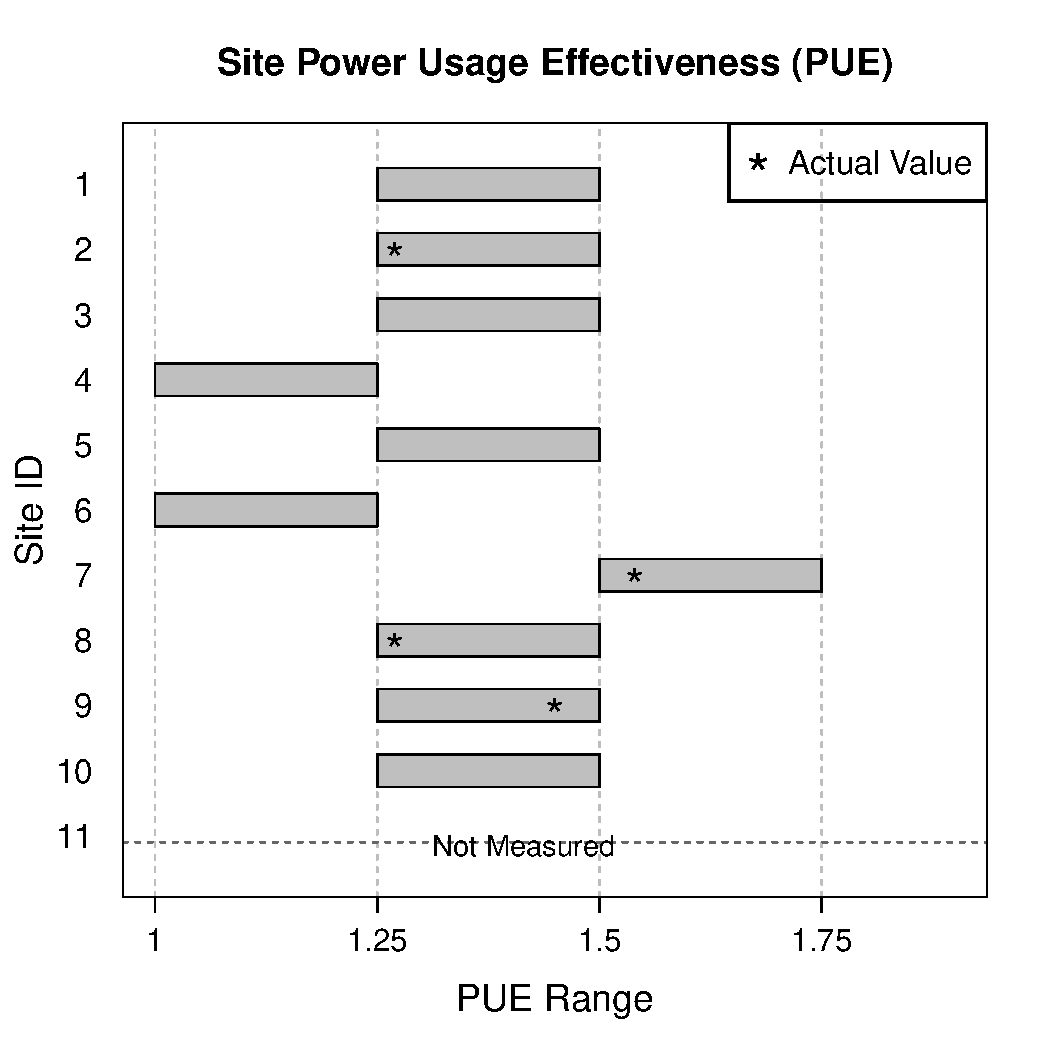
\includegraphics[scale=0.45]{NewGraphs/PUE-Graph.pdf}
\caption{Site Power Usage Effectiveness}
\label{figPUE}
\end{center}
\end{figure}

An open-ended question was posed as to whether or not there was information
either requested of the SCs by their ESPs or,
conversely, requested of the ESPs by the SCs. In both cases, well
over 75{\%} of the respondents answered no. LLNL and LANL were the
exceptions. LLNL is ``responding to requests for additional data on an hourly, 
weekly and monthly basis." They are also working to develop an automated capability to share 
data with their ESPs, which would provide automated additional 
detailed forecasting and ultimately real time data."
LANL has also been requested to provide average ``power projections, hour by hour,
for at least a day in advance.'' Additionally, LANL has asked their ESP for
more information on ``sensitivity of power distribution grid to rapid
transients (random daily step changes of 10 MW up or down within a single AC
cycle).''

Given the low levels of current engagement between the ESPs and the SCs, it is not surprising that none of
the SCs are currently using any power management
strategies to respond to grid requests by their ESPs. SDSC's \textit{supercomputer center} is not an exception, but they did respond that their
entire ``campus is leveraging parallel electrical distribution to trigger
diesel generators and other back-up resources to respond to grid and
non-grid requests.''

It was suggested by ORNL that some of the power management strategies 
are of questionable business value even for energy efficiency, let alone grid integration.
For example, ORNL comments that ``these assets have very clear depreciation schedules, and the modest cost 
savings in terms of electricity consumption due to some of these methods may not (or frequently will not) 
outweigh the capital investment cost in the computer. That is, if a site spent \$100M for a computer that will 
remain in production for 60 months, then the 
apparent benefit of power capping, etc can easily be outweighed by lost productivity of the consumable resource.

Similarly, another comment by ORNL suggested that the rapid deployment of hardware features, like P-states,  may outpace the need for strategies like power aware job scheduling.

We tried to evaluate if power management strategies will be considered
relevant and effective for grid integration at some point in the future. Two
questions were asked: is there interest in using the strategies and what
impact did they think that the strategies would have? When combining
interest and impact, the results showed that power capping, shutdown, and
job scheduling were both potentially interesting and of high impact (see Table \ref{tab3}). 

Load migration, back-up
scheduling, fine-grained power management and thermal management were of medium
interest and impact. Lighting control and back-up resources were of low
interest and impact. 

Temperature control and lighting management are utilized as strategies, but considered medium to low interest and impact
for responding to requests from ESPs. 
The infrastructure energy efficiency of the responding supercomputer sites is high, as reflected in their reported
Power Usage Effectiveness (PUE) (Figure \ref{figPUE}). Two sites reported a PUE below 1.25, the majority were between 
1.25 and 1.5 and the highest was 1.53. Approximately half of the respondents said that they used 
temperature control and lighting management
as strategies, but not for grid requests. Temperature control and lighting management are well documented and understood
strategies for improving energy efficiency, so it is not surprising that sites with PUEs below 1.5 are using them.

NOAA comments that their ``lights automatically shut off 24x7 
when there is no motion in the data center." There is a value in lighting control for 
energy efficiency purposes, as demonstrated by its having been fully implemented. NOAA also comments that
the impact of further lighting control ``is so small compared to the HPC demand load that" they would ``be surprised 
if the utility is interested.''

LLNL reports that they ``took 3 years to raise the temperature in their center by 18 degrees F. It was done in conjunction with a failure rate analysis of the systems as well as a measurement of the electrical savings prior to moving to the next set point.'' LLNL is currently operating in the ASHRAE 
recommended range, but expresses concerns with increasing temperature as a grid-integration response. The 
concerns include hardware failures, 
tape storage read/write errors and compromising dew point requirements where liquid and air-cooling are co-located.

Distinguishing interest from impact sheds further insight; some strategies are 
considered high impact, but not interesting enough to consider deployment. Facility
shutdown is rated as having a high impact, but only
considered interesting by 36\% of the respondents. NOAA commented that, ``We've had too many HPC
instability and equipment failures to utilize this as a strategy." This divide is even more
apparent with load migration. It is rated as having a high impact by 36\% of the
respondents, but only interesting to 10\%. 
